\documentclass[a4paper]{article}
\newcommand\hmmax{0}
\newcommand\bmmax{0}
\usepackage{booktabs}

%% Language and font encodings
\usepackage[english]{babel}
\usepackage[utf8x]{inputenc}
\usepackage[T1]{fontenc}
\usepackage{gensymb}
\usepackage{pdfpages}

\usepackage[bitstream-charter]{mathdesign}
\let\circledS\undefined
%% Sets page size and margins
\usepackage[a4paper,top=2cm,bottom=2cm,left=1cm,right=5cm,marginparwidth=4cm]{geometry}

%% Useful packages
\usepackage{amsmath}
\usepackage{bm}
\usepackage[makeroom]{cancel}
\usepackage{enumitem}
\usepackage{listings}
\usepackage{multirow}
\usepackage{amssymb}
\usepackage{float}
\usepackage{graphicx}
\usepackage[colorinlistoftodos]{todonotes}
\usepackage[colorlinks=true, allcolors=blue]{hyperref}
\usepackage[final]{matlab-prettifier}
\usepackage{courier}
\usepackage{algorithm}
\usepackage[noend]{algpseudocode}
\usepackage[]{appendix}
\usepackage{wrapfig}
\usepackage[final]{matlab-prettifier}
\usepackage[final]{mathtools}

\newtheorem{theorem}{Theorem}[section]
\newtheorem{corollary}{Corollary}[theorem]
\newtheorem{lemma}[theorem]{Lemma}
\newtheorem{definition}[theorem]{Definition}


\renewcommand\labelitemi{$\bullet$}

\definecolor{codecol}{rgb}{0.94, 0.94, 0.94}
\definecolor{dgreen}{rgb}{0.1, 0.49, 0.1}

\newcommand{\ea}{\nonumber \\}
\lstset{basicstyle=\footnotesize\ttfamily,breaklines=true}
\lstset{framextopmargin=50pt,frame=bottomline}

\newcommand{\norm}[2]{\left\Vert#1\right\Vert_{#2}}
\newcommand{\question}[1]{{\color{red}\textbf{Question: }\emph{#1}}}
\newcommand{\action}[1]{{\color{blue}\textbf{Action: }\emph{#1}}}
\newcommand{\epdp}{$(\epsilon, \delta)$-DP}
\newcommand{\alg}{$\mathcal{A}$}
\newcommand{\data}{$\mathcal{D}$}
\newcommand{\vect}[1]{\boldsymbol{\mathbf{#1}}}
\newcommand{\normaldist}[2]{$\mathcal{N}(#1, #2)$}
\newcommand{\expt}[2]{\mathbb{E}_{#2}[#1]}
\newcommand{\prob}[2]{\mathbb{P}_{#2}[#1]}
\newcommand{\model}[1]{\mathcal{M}_{#1}}
\newcommand{\indep}{\raisebox{0.05em}{\rotatebox[origin=c]{90}{$\models$}}}
\newcommand{\mset}[3]{\lbrace {#1}_{#2} \rbrace_{#2=1}^{#3} }
\DeclarePairedDelimiter{\ceil}{\lceil}{\rceil}

\newcommand{\ix}[1]{%
  \leavevmode % if at the start of a paragraph
  \marginpar{\small\emph{#1}}% the note
}

\newcommand{\qx}[1]{%
	\leavevmode % if at the start of a paragraph
	\marginpar{\color{blue}\small\emph{#1}}% the note
}
\newcommand{\marfig}[2]{
  \marginpar{ \includegraphics[width=\marginparwidth]{#1} \centering \text{\small #2} }
}

\DeclareMathAlphabet{\altmathcal}{OMS}{cmsy}{m}{n}

\title{\textbf{4F3: Optimal and Predictive Control}\\
\textit{Need to Know}
}
\author{Mrinank Sharma}

\begin{document}
\maketitle
% \tableofcontents
Please note that the margins of these notes can be used to check factual recall simply by covering up the right hand text.

\section{Introduction}
\ix{Convex Optimisation}A convex optimisation problem is written as follows:
\begin{align}
\min_x\ &f_0(x) \nonumber \\
\text{s.t.}\ &f_i(x) \leq b_i \hspace{1cm} i=1, \ldots, m \nonumber \\
&h_i(x) = 0 \hspace{1cm} i=1, \ldots, p
\end{align}
where the objective and inequality constraint functions are convex i.e. $f_i (\alpha x + \beta y) \leq \alpha f_i(x) + \beta f_i(y)$ and the equality constraint functions are linear plus a constant for $\alpha + \beta = 1$, $\alpha \geq 0$ and $\beta \geq 0$. 

\ix{Significance of Convex Optimisation} Whilst there is no analytical solution for this class of problems, there is a global minimum and there are reliable and efficient algorithms. There are many tricks for transforming problems into convex form. 

Notation:
\begin{align}
||y||_\infty &= \max_t \sqrt{y^T(t) y(t)} \\
||y||_2^2 &= \int_{-\infty}^\infty y^T(t) y(t) dt
\end{align}

\section{Optimal Control and Dynamic Programming}
\subsection{Discrete Time Finite Horizon Optimal Control}
State $x \in \altmathcal{X}$, input $u \in \altmathcal{U}$. Dynamics of the system are:
\begin{align}
x_{k+1} = f(x_k, u_k) \text{ where } f(\cdot, \cdot): \altmathcal{X} \times \altmathcal{U} \rightarrow \altmathcal{X}
\end{align}
\ix{Cost Function}Given an initial condition, the input sequence deterministically generates a state-sequence. The cost function, in general, over a finite horizon $h$ time-steps into the future, can be written as:
\begin{align}
J(x_0, u_0, \ldots, u_{h-1}) = \sum_{k=0}^{h-1} \underbrace{c(x_k, u_k)}_{\text{stage cost}} + \overbrace{J_h(x_h)}^{\text{terminal cost}}
\end{align}
Our objective is to find the input sequence which minimises the above cost function for a given initial state. Note: in certain cases, $J^*$ may not be well-defined and the optimal input sequence may not exist, or may be non-unique. 

\ix{Bellman's Principle of Optimality} Assume that the optimal control sequence, $u_0^*, \ldots, u_{h-1}^* $, leads us from $x_0$ to $x_k$ at step $k$. Then the truncated sequence $u_k^*, \ldots, u_{h-1}^*$ is a solution to the truncated problem:
\begin{align}
u_k^*, \ldots, u_{h-1}^* = \text{arg}\ \min_{u_k, \ldots, u_{h-1}} \sum_{i=1}^{h-1} c(x_i, u_i) + J_h(x_h)
\end{align}
\ix{Value Function}The \emph{Value Function} is defined as:
\begin{align}
V(x, k) \triangleq \min_{u_k, \ldots, u_{h-1}} \sum_{i=1}^{h-1} c(x_i, u_i) + J_h(x_h)
\end{align}
where $x_i, i>k$ is generated using the system dynamics. Also known as the \emph{cost-to-go}, this function is the optimal \emph{additional cost} from the $k$th step. 

Assume that $V(x, k+1)$ is known for all $x$. Then\qx{Proof: Value Function Recursion}
\begin{align}
V(x, k) = \min_{u_k} \Big \lbrace c(x, u_k) + V(x_{k+1}, k+1)  \Big \rbrace \label{eq:dynamic_programming}
\end{align}
Thus, the optimal control and cost can be found by solving the \emph{Dynamic Programming Equation} (Eq. \ref{eq:dynamic_programming}) starting with the final condition $V(x, h) = J_h(x)$. The optimal control is the sequence of $\lbrace u_k \rbrace$ minimising the cost at each stage of the dynamic programming equation. 

\ix{Comments} The magic of dynamic programming has converted a minimisation over $h$ inputs to a sequence of $h$ minimisations over one input. Solving this equation gives the optimal control for all values of $x_0$ over this horizon length. This can always be solved if the state and input can only take a finite number of values. 

\subsection{Discrete-Time Finite Horizon Linear Quadratic Regulator}
\ix{Discrete-time LQR}State $x \in \altmathcal{X}$, input $u \in \altmathcal{U}$. Dynamics of the system are:
\begin{align}
x_{k+1} = Ax_k + Bu_k
\end{align}
The initial condition, $x_0$, is assumed given. The cost function is
\begin{align}
J(x_0, u_0, \ldots, u_{h-1}) = \sum_{k=1}^{h-1} x_k^T Q x_k + u_k^T R u_k + x_h^T X_h x_h
\end{align}
$Q, R, X_h$ are symmetric matrices with $Q \geq 0$, $R > 0$ and $X_h \geq 0$. This implies that $R^{-1}$ exists. Therefore, for the penultimate time-step:
\begin{align}
V(x, h-1) &=  \min_{u} \Big \lbrace x^T Q x + u^T R u + (Ax + Bu)^{T} X_h (A_x+Bu))  \Big \rbrace \nonumber \\
&= x^{T} \underbrace{(Q + A^{T}X_h A - A^{T}X_h B(R + B^T X_h B)^{-1} B^T X_h A)}_{X_{h-1}}x
\end{align}
which is another quadratic form in $x$. Thus, the backwards difference equation
\begin{align}
X_{k-1} = Q + A^{T}X_k A - A^{T}X_k B(R + B^T X_k B)^{-1} B^T X_k A) \label{eq:lqr_backwards}
\end{align}
is solved, and the optimal control is found as the minimiser at each time-step: \qx{Prove the state feedback equation}
\begin{align}
u_k = -(R + B^T X_{k+1} B)^{-1} B^T X_{k+1} A x_k
\end{align}
which is state-feedback control. 

\subsection{Continuous Time Dynamic Programming}
State $x \in \mathbb{R}^n$, input $u \in \altmathcal{U} \subseteq  \mathbb{R}^m$. Dynamics of the system are:
\begin{align}
\dot{x} = f(x, u) \text{ where } f(\cdot, \cdot): \mathbb{R}^n\times \altmathcal{U} \rightarrow \mathbb{R}^n
\end{align}
Given $x_0 \in \altmathcal{X}$ and a horizon $T\geq 0$, each input function $u(\cdot): [0, T] \rightarrow \altmathcal{U}$ generates a state trajectory satisfying the above dynamics. \ix{Continuous Time: New Cost Function}The cost function is now:
\begin{align}
J(x_0, u(\cdot)) = \int_{0}^T c(x(t), u(t)) dt + J_t(x(T))
\end{align}
The aim is to find the best input function:
\begin{align}
u^*(\cdot) = \arg \min_{u(\cdot)} J(x_0, u(\cdot))
\end{align}
Technical assumptions are placed on $f, \altmathcal{U}, c, J_h$ to ensure that a unique trajectory exists, a unique optimal control exists and that there is a minimum of the cost function. 

\ix{Bellman Optimality: Continuous Time} Assumption that the optimal control $u^*(\cdot): [0, T] \rightarrow \altmathcal{U}$ leads from $x(0)$ to $x(t)$ at $t < T$. Then the truncated control $u^*(\cdot): [t, T] \rightarrow \altmathcal{U}$ is a solution to the truncated problem:
\begin{align}
\min_{u(\cdot)} \int_{t}^T c(x(\tau), u(\tau)) d\tau + J_t(x(T))
\end{align}

\ix{Value Function}The value (or cost-to-go) function $V: \altmathcal{X} \times [0, T] \rightarrow \mathbb{R}$ is defined as:
\begin{align}
V(x(t), t) \triangleq \min_{u(\cdot)} \int_{t}^{T} c(x(\tau), u(\tau)) d\tau + J_t(x(T))
\end{align}
\qx{Derive Value Function PDE}The recursive algorithm in discrete-time is converted to a partial differential equation known as the \emph{Hamilton-Jacobi-Bellman PDE}:
\begin{align}
- \frac{\partial V(x, t)}{\partial t} = \min_{u(\cdot)} \Big \lbrace  c(x, u) + \frac{\partial V(x, t)}{\partial x} f(x, u) \Big \rbrace
\end{align}
Solving the above PDE with condition $V(x, T) = J_t(x)$ yields the solution. The optimal cost is given by $V(x_0, 0)$ and the optimal input is:
\begin{align}
u^*(t) = \arg \min_{u \in \altmathcal{U}} \Big \lbrace c(x(t), u) + \frac{\partial V(x, t)}{\partial x} f(x(t), u)\Big \rbrace
\end{align}
The optimisation over $u(\cdot)$ has been converted to a pointwise optimisation over $u \in \altmathcal{U}$. \textbf{Note: } to solve the problem, a PDE needs to be solved, but there can be technical difficulties with this e.g. does a solution exist, and if so, in what sense? It is computable? 

\subsection{Continuous-Time LQR}
$x \in \mathbb{R}^n, u \in \mathbb{R}^m, x(0) = x_0$. Horizon of $t_1$. System dynamics are:
\begin{align}
\dot{x} = Ax + Bu
\end{align}
The cost function is:
\begin{align}
J(x_0, u(\cdot)) = \int_{0}^{t_1} x^T Q x + u^T R u\  dt\ + x(T)^T X_{t_1} x(T)
\end{align}
with $R = R^{T} > 0$, $Q = Q^{T} \geq 0$ and $X_{t_1} = X_{t_1}^{T} \geq 0$. \ix{Value Function Form}. Let $V(x, t) = x^T X(t) x$. Defining the vector gradient as a row vector, the HJB reads: \qx{Fill in the missing steps...}
\begin{align}
-x^T \dot{X}(t) x &= \min_{u} \Big\lbrace x^T Q x + u^T R u + 2x^T X(t)(Ax + Bu)  \Big\rbrace \nonumber \\
&= x^T (Q+ XA + A^{T}X - XBR^{-1}B^{T}X)x \\
u^*(t) &= -R^{-1}B^T X(t) x(t)
\end{align}
\ix{Riccati Equation}Thus, the following ODE (a \textbf{Riccati equation}) must be solved \emph{backwards in time}
\begin{align}
-\dot{X} = Q+ XA + A^{T}X - XBR^{-1}B^{T}X \label{eq:lqr-riccati}
\end{align}
with terminal condition $x_0^T X(0) x_0$. Solving the value function backwards allows the optimal control function to be found, which is the then integrated forwards. \ix{Empirical Findings} It is found that when simulating the solution to the Riccati equation backwards in time, the terminal cost causes a transient, beyond which (i.e. earlier in time) the matrix $X$ appears to converge in value. 

\subsection{Infinite Horizon Continuous Time LQR}
\ix{Setup}The problem is setup with 
\begin{align}
\dot{x} = Ax + Bu \hspace{1cm}
x(0) &= x_0 \hspace{1cm}
z = \begin{bmatrix}
Cx \\ u 
\end{bmatrix}\nonumber
\end{align}
The cost function is defined as:
\begin{align}
J(x_0, u(\cdot)) &= \int_0^{\infty} z(t)^T z\ dt
\end{align}
\ix{Technical Assumptions} It is assumed that $(A, B)$ is controllable and $(A, C)$ is observable. \ix{Intuition} The infinite horizon is like a finite, but very long horizon. The solution is given by the Riccati equation:
\begin{align}
-\dot{X} = C^T C + XA + A^{T}X - XBR^{-1}B^{T}X
\end{align}
for \textbf{any} final condition, as it does not have a large effect for long times. Therefore, we expect that: 
\begin{align}
u^*(t) &= - B^T X x(t) \\
\dot{x} &= Ax + Bu = (A - BB^T X)x
\end{align}
where $X = X^T$ solves the \emph{Control Algebraic Riccati Equation (CARE)}:
\begin{align}
C^T C + XA + A^{T}X - XBR^{-1}B^{T}X = 0
\end{align}
It can be shown that the CARE has a unique, symmetric, positive definite solution $X = X^T \geq 0$ and this this solution is stabilising i.e. $A - BB^T$ has all eigenvalues in the left half plane. This solution can be obtained as $\lim_{t\rightarrow -\infty} X(t)$ where $X(t)$ solves Eq. \ref{eq:lqr-riccati} for \textbf{any} final condition. 

\ix{Alternative Derivation} Let $X = X^T$ be the stabilising solution to the CARE. Defining $V(t) = x(t)^T X x(t)$ and integrating $\dot{V} + z^T z$ gives, for matrix $X$ solving the CARE:
\begin{align}
V(\infty) - V(0) + ||z||_2^2 = || u + B^T X x ||_2^2
\end{align} 
Assuming $x(t) \rightarrow 0$ as $t \rightarrow \infty$, meaning that $V(\infty) = 0$, we have:
\begin{align}
\underbrace{||z||_2^2}_{J(x(0), u(\cdot))} = x(0)^T X x(0) + \underbrace{|| u + B^T X x ||_2^2}_{0\text{ if } u=-B^T X x} \label{eq:inf_horizon_lqr}
\end{align}

\section{$\altmathcal{H}_2$ Optimal Control}
\subsection{The $\altmathcal{H}_2$ norm}
\begin{definition}[$\altmathcal{H}_2$ norm] The $\altmathcal{H}_2$ norm of a system defined by its matrix transfer function, $G(s)$, is defined as:
	\begin{align}
	||G||_2^2 = \int_{-\infty}^\infty \text{trace} \lbrace G(j \omega)^* G(j\omega) \rbrace d\omega
	\end{align}
\end{definition}
\ix{Properties of the $\altmathcal{H}_2$ norm}Therefore:\begin{align}
||G||_2^2 = \sum_i ||G_i||_2^2
\end{align}
Assuming that $G(s)$ is a transfer function from $u$ to $y$, it can be shown that:
\begin{align}
||y||_\infty \leq \frac{1}{\sqrt{2\pi}} ||G||_2 ||u||_2
\end{align}
Consider the stable linear system
\begin{align*}
\dot{x} = Ax + Bu \hspace{1cm} y=Cx
\end{align*}
with transfer function $G(s) = C(sI - A)^{-1}B$. It can be shown that: \begin{align}
\frac{1}{\sqrt{2\pi}} ||G(s)||_2 &= \sqrt{\text{trace}(B^T L B)}  \nonumber\\
\text{where }L&=L^T\text{ solves } AL + LA + C^TC = 0
\end{align}  

\subsection{Linear Fractional Transformations}
\emph{Linear Fractional Transformations} are a useful way of manipulating close-loop transfer functions and approach norm-optimal control problems. 
\begin{definition}
	The\marfig{figs/lft}{} lower LFT $\altmathcal{F}_l(P(s), K(s))$ is defined as the closed loop transfer function from $\bar{w}(s)$ to $\bar{z}(s)$ i.e.
	\begin{align}
	\altmathcal{F}_l(P(s), K(s)) = T_{\bar{w} \rightarrow \bar{z}}
	\end{align}
\end{definition}
$P(x)$\ix{Generalised Plant} is known as the \emph{Generalised Plant} and has the following block transfer function representation:
\begin{align}
\begin{bmatrix}
\bar{z}(s) \\ \bar{y}(s)
\end{bmatrix} =
\underbrace{\begin{bmatrix}
	P_{11}(s) & P_{12}(s) \\
	P_{21}(s) & P_{22}(s)
	\end{bmatrix}}_{P(s)} \begin{bmatrix}
\bar{u}(s) \\ \bar{w}(s)
\end{bmatrix}
\end{align}
\ix{Interpreting $w$ and $z$}Note that $w$ usually represents some sort of control input, for example, driving disturbance noise, either in output or state. $z$ is the control output and typically represents some sort of performance measure.  

\qx{Show form of LFT}Note that it can be shown that:
\begin{align}
\altmathcal{F}_l(P(s), K(s)) = P_{11}(s) + P_{12}(s)K(s)(I - P_{22}(s) K(s))^{-1} P_{21}(s)
\end{align}

\subsection{$\altmathcal{H}_2$ Optimal State Feedback Control}
Consider the following generalised plant:\ix{Plant Setup}
\begin{align}
\begin{bmatrix}
\dot{x} \\ z \\ y
\end{bmatrix} = \begin{bmatrix}
A & B_1 & B_2 \\ 
\begin{bmatrix}
C_1 \\ 0
\end{bmatrix}  & 0 & \begin{bmatrix}
0 \\ I
\end{bmatrix} \\
I & 0 & 0
\end{bmatrix} \begin{bmatrix}
x \\ w \\ u
\end{bmatrix}
\end{align}
$w$ represents an external disturbance and $z$ penalises deviations from $0$ in the state and using input energy. Note that since $y = x$, this is state feedback i.e. the controller has \textbf{direct access to the state}. We make the technical assumptions that the pair $(A, B_2)$ is controllable and $(A, C_1)$ is observable. 

\ix{Objective}The objective is as follows:
\begin{align}
\min_{K(s)\text{ stabilising}} ||\altmathcal{F}_l(P(s), K(s))||_2 = \min_{K(s)\text{ stabilising}} \sqrt{2\pi} \sqrt{\sum_i \Big|\Big| z(t)|_{w(t) = e_i \delta(t)}   \Big|\Big|_2^2 }
\end{align}
Choose $X = X^T$ as the stabilising solution to the CARE equation. Setting $\bar{u}(s) = \underbrace{-B_2^T X}_{K(s)} \bar{x}(x)$ gives the optimal solution:
\begin{align}
\frac{1}{2\pi} ||\altmathcal{F}_l(P(s), K(s))||_2^2  = \text{trace}(B_1^{T} X B_1)
\end{align}

\subsection{$\altmathcal{H}_2$ Optimal Output Feedback Control}
\ix{Problem Setup}The driving noise, $w_1$, is now considered with observation noise, $w_2$, altering the generalised plant, $P$. 
\begin{align}
\begin{bmatrix}
\dot{x} \\ z \\ y
\end{bmatrix} = \begin{bmatrix}
A & \begin{bmatrix}
B_1 & 0
\end{bmatrix} & B_2 \\ 
\begin{bmatrix}
C_1 \\ 0
\end{bmatrix}  & 0 & \begin{bmatrix}
0 \\ I
\end{bmatrix} \\
C_2 & \begin{bmatrix}
0 & I
\end{bmatrix} & 0
\end{bmatrix} \begin{bmatrix}
x \\ w \\ u
\end{bmatrix}
\end{align}
In addition to the prior assumptions (controllable $(A, B_2)$ and observable $(A, C_1)$), the additional assumptions that $(A, B_1)$ is controllable and $(A, C_2)$ is observable are made. This assumptions are appropriate for the dual problem. 

\subsection*{Derivation}
Choose $Y = Y^T$ as the stabilising solution (i.e. $A - YC_2^TC_2$ has eigenvalues in the LHP) to the \textbf{Filter Algebraic Riccati Equation(FARE)}\ix{FARE}:\begin{align}
0 = YA^T + AY + B_1 B_1^T - Y C_2^T C_2 Y
\end{align}
Now consider the observer. The system dynamics are:
\begin{align}
\dot{\tilde{x}} &= A^T \tilde{x} + F^T \tilde{w} + C_2^T \tilde{u} \\
\tilde{y} &= B_2^T \tilde{x} + \tilde{w}
\end{align}
Thus, setting
\begin{align}
\dot{\tilde{x}}_k = A^T \tilde{x}_k + F^T (\tilde{y} - B_2^T \tilde{x}_k) + C_2^T \tilde{u}
\end{align}
gives $\tilde{x}_k = \tilde{x} \Rightarrow \dot{\tilde{x}}_k = \dot{\tilde{x}}$, so provided the initial condition is the same for both, the observer trackers $\tilde{x}$. Then to minimise the additional cost, set
\begin{align}
\tilde{u} = -\underbrace{C_2 Y}_{H^T} \tilde{x}_k
\end{align}
Therefore, the optimal $K^T$ has the realisation:
\begin{align}
\begin{bmatrix}
\dot{\tilde{x_k}} \\
\tilde{u}
\end{bmatrix}
= \begin{bmatrix}
A^T - F^T B_2^T - C_2^T H^T & F \\
-H^T & 0
\end{bmatrix}\begin{bmatrix}
\tilde{x_k} \\
\tilde{y}
\end{bmatrix}
\end{align}
which gives the following optimal $K$. 
\begin{align}
\begin{bmatrix}
\dot{x_k} \\
u
\end{bmatrix}
= \begin{bmatrix}
A - B_2 F - HC_2 & -H \\
F & 0
\end{bmatrix}\begin{bmatrix}
x_k \\
y
\end{bmatrix}
\end{align}
Note that there is an alternative realisation of this $K$ which can be implemented in observer form. 

Thus, nothing that the initial steps of the output feedback derivation remain valid, the optimal $K$ achieves:
\begin{align}
\min_{K(s)\text{ stabilising}} ||\altmathcal{F}_l(P(s), K(s))||_2 = \sqrt{2\pi } \sqrt{\text{trace}(B_1^{T} X B_1)} + \sqrt{2\pi } \sqrt{\text{trace}(F Y F^T)}
\end{align}
The closed loop poles are\ix{Closed Loop Poles} $\lambda_i (A - B_2F) \bigcup \lambda_i (A - H C_2) $

\section{$\altmathcal{H}_\infty$ Optimal Control}
\subsection{$\altmathcal{H}_\infty$ Norm}
\begin{definition}
	The $\altmathcal{H}_\infty$ norm of a stable linear system, $G(s)$, between signals $u$ and $y$ has two interpretations:
	\begin{enumerate}[label=(\alph*): ]
		\item The Maximum Singular Value of $G(j\omega)$ i.e.
		\begin{align}
		||G||_{\infty} = \max_\omega \bar{\sigma}(G(j\omega))
		\end{align}
		\item Signal Energy Bound:
		\begin{align}
		||G||_{\infty} = \max_{\hat{u} \neq 0} \frac{||G \hat{u}||_2}{||\hat{u}||_2} = \max_{u \neq 0} \frac{||y||_2}{||u||_2}
		\end{align}
	\end{enumerate}
\end{definition}
\ix{Calculating the $\altmathcal{H}_\infty$ norm}Consider the system:
\begin{align}
\dot{x} &= Ax + Bu \nonumber\\
y &= Cx
\end{align}
with $x(0) = 0$. If (and only if) the Riccati equation:
\begin{align}
A^TX + XA + C^TC + \frac{1}{\gamma^2} XBB^TX = 0
\end{align}
has a solution, $X = X^T > 0$, then $||G||_\infty \leq \gamma$. This condition can be checked easily algebraically, so a bisection algorithm can be used to find the smallest value of $\gamma$ which has a solution to this equation with would be the $\altmathcal{H}_\infty$ norm.  

\subsection{$\altmathcal{H}_\infty$ Optimal Control}
Consider the\ix{Problem Setup} generalised plant with realisation:
\begin{align}
\begin{bmatrix}
\dot{x} \\ z \\ y
\end{bmatrix} =\begin{bmatrix}
A & \begin{bmatrix}
B_1 & 0
\end{bmatrix} & B_2 \\
\begin{bmatrix}
C_1 \\ 0
\end{bmatrix} & 0 & \begin{bmatrix}
0 \\ I
\end{bmatrix} \\
C_2 & \begin{bmatrix}
0 & I
\end{bmatrix} & 0
\end{bmatrix}\begin{bmatrix}
x \\ w \\ u
\end{bmatrix}
\end{align}
It is assumed that $(A, B_2)$ is controllable and $(A, C_2)$ is observable, which are appropriate to the state-feedback problem. Additionally, we assume that $(A, B_1)$ is controllable and $(A, C_2)$ is observable, appropriate for the estimation problem. Note: \textbf{we will also assume that} $x(0) = 0$. 

\ix{Objective}The objective is to find a stabilising controller, $K(s)$ such that 
\begin{align}
||\altmathcal{F}_l(P(s), K(s))||_\infty \leq \gamma
\end{align}
Consider $V = x^TX x$ for some $X=X^T$. Then:
\begin{align}
\frac{dV}{dt} + z^T z - \gamma^2 w^T w  =\ \nonumber &x^T (A^TX + XA + C^TC + \frac{1}{\gamma^2}  XBB^TX)x \nonumber \\
&+ (u + B_2^TXx)^T (u + B_2^TXx)  \nonumber\\ 
&-\gamma^2\Bigg( w - \frac{1}{\gamma^2} \begin{bmatrix}
B_1^T \\ 0
\end{bmatrix}Xx \Bigg)^T\Bigg( w - \frac{1}{\gamma^2} \begin{bmatrix}
B_1^T \\ 0
\end{bmatrix}Xx \Bigg)
\end{align}
\ix{Choosing $X$}Now, if $X=X^T$ is chosen to satisfy:
\begin{enumerate}[label=(\alph*): ]
	\item $A^TX + XA + C^TC + \frac{1}{\gamma^2}  XBB^TX = 0$.
	\item Closed loop stability in the absence of disturbance i.e. when $u = -B_2^TXx$ with $u=0$ meaning that $A - B_2B_2^T X$ (the closed loop `$A$' matrix) is stable.
	\item Closed loop stability in the worst case disturbance i.e. $A - B_2B_2^T X + \gamma^{-2} B_1B_1^T X$ stable. This occurs when:
	\begin{align}
	u &= -B_2^T Xx \nonumber \\
	w &= \frac{1}{\gamma^2} \begin{bmatrix}
	B_1^T \\ 0
	\end{bmatrix}Xx \nonumber
	\end{align}
\end{enumerate}
Note at most one solution to (a) also satisfies (c) and if there exists a stabilising $K(s)$ with the desired $\altmathcal{H}_\infty$ norm, then a solution to these equations exists. Choosing this $X$ and integrating yields:
\begin{align}
||z||_2^2 - \gamma^2 ||w||_2^2 = \Big|\Big| \underbrace{u + B_2^T Xx}_{v}\Big|\Big|_2^2 - \gamma^2 \Bigg|\Bigg| \underbrace{  w - \frac{1}{\gamma^2} \begin{bmatrix}
	B_1^T \\ 0
	\end{bmatrix}Xx}_{r} \Bigg|\Bigg|_2^2
\end{align}
since $x(\infty) = x(0) = 0$. 

\ix{State Feedback}If we are able to choose $u = -B_2^TXx$, then we immediately have $||T_{w \rightarrow z}||_\infty \leq \gamma$ noting the signs in the above equation. 

\ix{Output Feedback}However, if we cannot take $u = -B_2^TXx$, note that $||\altmathcal{F}(P, K)||_\infty \leq \gamma \Rightarrow ||T_{r \rightarrow v}||_\infty \leq \gamma$. 

\subsection*{Output Feedback Derivation}
\ix{Optimal Observer}Consider:
\begin{align}
\dot{\tilde{x}}_k = \hat{A}^T \tilde{x}_k + F^T \underbrace{(\tilde{y} - B_2\tilde{x}_k)}_{\tilde{r}_\text{est}} - C_2^T C_2 Y\tilde{x}_k
\end{align}
For this system, $\tilde{x}_k = \tilde{x} \Rightarrow \dot{\tilde{x}}_k = \dot{\tilde{x}}$. Define $H^T = C_2 Y$. The following optimal $K$ is. 
\begin{align}
\begin{bmatrix}
\dot{x_k} \\
u
\end{bmatrix}
= \begin{bmatrix}
\hat{A} - B_2 F - HC_2 & -H \\
F & 0
\end{bmatrix}\begin{bmatrix}
x_k \\
y
\end{bmatrix}
\end{align}

\section{Convex Optimisation \& LMIs for Control Design}
Consider the stable linear system, $G(s)$, with state-space realisation:
\begin{align}
\dot{x} &= Ax + Bu \nonumber \\
y &= Cx
\end{align}
Stability of the system can be shown by finding $V = x^TXx, X=X^T > 0$ such that $\dot{V} < 0$ for $u = 0$ i.e. by finding a \emph{Lyapunov function} since $V(x(t)) \rightarrow 0$ as $t \rightarrow \infty$ implies $x(t) \rightarrow 0$. This is equivalent to:
\begin{align}
\dot{V} = x^T(A^T X + XA)x < 0 \Leftrightarrow A^T X + XA < 0
\end{align}
This is a \emph{Linear Matrix Inequality (LMI)}. 

Note that:
\begin{align}
Q \geq 0 \text{ iff } R^T Q R \geq 0
\end{align} 
for any invertible matrix $R$. This then gives\ix{Schur Complement}:
\begin{align}
\begin{bmatrix}
Q & S \\ S^T & R
\end{bmatrix} \geq 0 \hspace{0.5cm} \text{iff} \hspace{0.5cm} R \geq 0 \text{ and } Q - SR^{-1}S^T \geq 0
\end{align} 
provided $Q = Q^T$ and $R = R^T$ is invertible. \qx{Proof of Schur Complement}This is easy to show by considering:
\begin{align}
\begin{bmatrix}
I & 0 \\-R^{-1}S^T & I
\end{bmatrix}^T \begin{bmatrix}
Q & S \\ S^T & R
\end{bmatrix} 
\begin{bmatrix}
I & 0 \\-R^{-1}S^T & I
\end{bmatrix}
\end{align}
There exist efficient algorithms to solve LMIs. 

\subsection{Design of Stabilising Controllers}
Consider the system:
\begin{align}
\dot{x} &= Ax + Bu \nonumber\\
u &= Kx
\end{align}
As before, we seek $X = X^T > 0$ and $K$ such that $V = x^T X x$ and $\dot{V} < 0$. \ix{First Inequality}This is equivalent to finding:
\begin{align}
(A+BK)^TX + X(A+BK)\leq 0
\end{align}
However, this is not a LMI as there are terms corresponding to the product of $K$ and $X$.\qx{Convert to LMI} To convert this into an LMI, multiply left and right by $Y = X^{-1}$ and write $Z = KY$. We then form the following LMI:
\begin{align}
YA^T + Z^T B^T + AY + BZ \leq 0
\end{align}
After solving for $Y$ and $Z$, then $X = Y^{-1}$ and $K = ZX$. 

\subsection{$\altmathcal{H}_\infty$ Optimal Control}
\ix{Computing the $\altmathcal{H}_\infty$ norm}Consider the system $G$ represented as follows:
\begin{align}
\dot{x} &= Ax + Bu + B_w w \nonumber\\
z &= Cx
\end{align}
From the previous section, $||G||_\infty \leq \gamma$ if for some $X=X^T > 0$, $V = x^T X x$ satisfies:
\begin{align}
\dot{V} + z^Tz - \gamma^2 w^T w \leq 0
\end{align}
This can be written as a LMI:\qx{Show this Expression}
\begin{align}
\begin{bmatrix}
x \\ w
\end{bmatrix}^T \begin{bmatrix}
A^TX + XA + C^T C & XB_w \\
B_w^T X & -\gamma^2 I
\end{bmatrix}
\begin{bmatrix}
x \\ w
\end{bmatrix} \leq 0
\end{align}
Thus to compute $||G||_\infty$, find $X=X^T$ and $\min \gamma$ such that:
\begin{align}
\begin{bmatrix}
A^TX + XA + C^T C & XB_w \\
B_w^T X & -\gamma^2 I
\end{bmatrix} \leq 0
\end{align}

\ix{Computing the Optimal State-Feedback Controller}
For the system: \begin{align}
\dot{x} &= Ax + Bu + B_w w \nonumber\\
z &= Cx + Du 
\end{align}
we want to find a controller, $u=Kx$ that minimises $||T_{w\rightarrow z}||_\infty$. Applying the same trick as usual yields:
\begin{align}
\begin{bmatrix}
(A+BK)^TX + X(A+BK) + (C+DK)^T(C+DK)& XB_w \\
B_w^T X & -\gamma^2 I
\end{bmatrix} \leq 0
\end{align}
However, this is not a LMI. Multiplying left and right by $\begin{bmatrix}
Y & 0 \\ 0 & I
\end{bmatrix}$ gives:
\begin{align}
\begin{bmatrix}
Y(A+BK)^T + (A+BK)Y + Y(C+DK)^T(C+DK)Y& B_w \\
B_w^T  & -\gamma^2 I
\end{bmatrix} \leq 0
\end{align}
Then, clearly:
\begin{align}
\begin{bmatrix}
Y(A+BK)^T + (A+BK)Y + Y(C+DK)^T(C+DK)Y& 0 & B_w \\
0 & -I & 0 \\
B_w^T  & 0 & -\gamma^2 I
\end{bmatrix} \leq 0
\end{align}
Then, applying the Schur complement:
\begin{align}
\begin{bmatrix}
Y(A+BK)^T + (A+BK)Y & Y(C+DK)^T & B_w \\
(C+DK)Y & -I & 0 \\
B_w^T  & 0 & -\gamma^2 I
\end{bmatrix} \leq 0
\end{align}
As before, write $Z = KY$ to give:
\begin{align}
\begin{bmatrix}
YA^T+Z^TB^T + AY+BKZ & YC^T+Z^TD^T & B_w \\
CY+DZ & -I & 0 \\
B_w^T  & 0 & -\gamma^2 I
\end{bmatrix} \leq 0
\end{align}
which is a LMI in $Y$ and $Z$. Similarly, solve for $Z$ and $Y$, then use these to calculate $X = Y^{-1}$ and $K = ZY^{-1} = ZX$. Note that we are also minimising over $\gamma$. 

\chapter{Predictive Control}
\section{Introduction to Predictive Control}
\emph{Predictive Control} is a different approach to control; the control input to the plant is the solution to an optimisation problem computed at discrete time-steps. The advantages of predictive control include:
\begin{enumerate}
	\item Systematic method of handling constraints. 
	\item Can operate close to constraints. 
	\item Easy to tune. 
\end{enumerate} 
All systems have constraints, such as physical constraints (e.g. an actuator limit), a safety constraint or a performance constraint. 

\ix{How does Predictive Control Work}Predictive control works as follows. At each sampling instant, a predictive controller:
\begin{enumerate}
	\item Takes a measurement of the system state. 
	\item Computes a sequence of inputs over a finite time horizon using an internal model to predict states are future times and minimising some cost function of future states and inputs. The controller checks that no constraints are violated on states and inputs. 
	\item Implements the first part of the optimal sequence. 
\end{enumerate} 
Note that this is a feedback control law. Each new measurement is used to calculate a new input, and the prediction horizon recedes over time. 
\begin{figure}
	\centering
	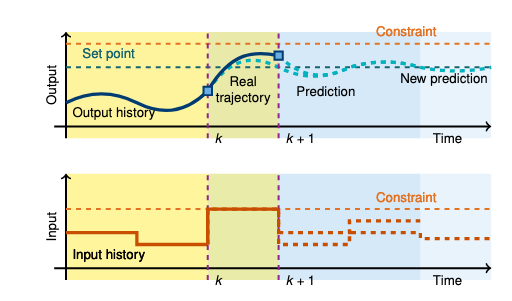
\includegraphics[width=0.5\textwidth]{figs/red_horizon}
	\caption{Receding Horizon Principle}
\end{figure}
\ix{Compared to Optimal Control}For example, with a linear model, quadratic costs without constraints, this is exactly a LQR problem, but optimisation occurs directly in the loop in real time. Note that the choice of cost function is more flexible, and that typically the optimisation is constrained. 

However, there is no guarantees about performance or stability in the long run. 

\section{Unconstrained Predictive Control}
Consider a discrete time system:
\begin{align}
x(k+1) = Ax(k) + Bu(k)
\end{align}
\ix{Assumptions}It is assumed that we can apply full state feedback (i.e. we have state measurements). The goal is to regulate states around the origin and there are no delays, noise, disturbances, model errors etc. 

\ix{Task}In this situation, the task is to find the finite horizon input sequence with minimises the finite horizon cost function:
\begin{align}
V(x, u_0, \ldots, u_{N-1}) = \sum_{i=0}^{h-1} \Big( x_i^T Q x_i + u_i^T R u_i \Big) + x_N^T P x_N
\end{align}
$R > 0$ penalises non-zero inputs, $Q \geq 0$ penalises non-zero states. This is precisely the LQR problem, and thus the receding horizon controller with state feedback is:
\begin{align}
u = -(R + B^T X_{1} B)^{-1} B^T X_{k+1} A x_1
\end{align}
where $X_1$ is found by solving a backwards difference equation. 

\ix{Alternative Derivation}Recalling the dynamics of the system, note that:
\begin{align}
x_i = A^i x_0 + A^{i-1}Bu_0 + A^{i-2}Bu_1 + \ldots Bu_{i-1}
\end{align}
Define the stacked vectors, $\vect{u} \in \mathbb{R}^{Nm}$ and $\vect{x} \in \mathbb{R}^{Nn}$
\begin{align}
\vect{u} = \begin{bmatrix}
u_0 \\ u_1 \\ \vdots \\ u_{N-1}   
\end{bmatrix} \hspace*{1cm} \vect{x} = \begin{bmatrix}
x_1 \\ x_2 \\ \vdots \\ x_{N}   
\end{bmatrix}
\end{align}
Then:
\begin{align}
\underbrace{\begin{bmatrix}
	x_1 \\ x_2 \\ \vdots \\ x_{N}   
	\end{bmatrix}}_{\vect{x}} = \underbrace{\begin{bmatrix}
	A\\ A^2 \\ \vdots \\ A^{N}
	\end{bmatrix}}_{\Phi} x_0 + \underbrace{\begin{bmatrix}
	B & 0 & \cdots & 0 \\
	AB & B & \cdots & 0 \\
	\vdots & \vdots & \ddots & \vdots \\
	A^{N-1}B & A^{N-2}B & \cdots & B
	\end{bmatrix}}_{\Gamma} \underbrace{\begin{bmatrix}
	u_0 \\ u_1 \\ \vdots \\ u_{N-1}   
	\end{bmatrix}}_{\vect{u}}
\end{align}
i.e. $\vect{x} = \Phi x_0 + \Gamma \vect{u}$. 

The cost function can be written as:
\begin{align}
V(x, \vect{u}) &= x_0^T Q x_0 + \vect{x}^T \underbrace{\begin{bmatrix}
	Q & &  & \\
	&  \ddots & & \\
	&  & Q & \\ 
	&   & &  P\\
	\end{bmatrix}}_{\Omega} \vect{x} + \vect{u}^T \underbrace{\begin{bmatrix}
	R & &  & \\
	&  R & & \\
	&  & \ddots & \\ 
	&   & &  R\\
	\end{bmatrix}}_{\Psi} \vect{u} \\
&= x^T Q x + \vect{x}^T\Omega \vect{x} + \vect{u}^T\Psi \vect{u}
\end{align}
Note that $\Omega \geq 0$ and $\Psi > 0$ due to the assumptions placed on $Q, P$ and $R$. Substituting in yields:
\begin{align}
V(x, \vect{u}) = \frac{1}{2} \vect{u}^T \underbrace{\Big \lbrace 2\Psi + 2\Gamma^T \Omega \Gamma \Big \rbrace}_{G} \vect{u} + \vect{u}^T \underbrace{\Big \lbrace 2\Gamma^T \Omega \Phi \Big \rbrace}_{F} \vect{x} + x^T(Q + \phi^T \Omega \phi)x
\end{align}
which is a quadratic cost, which has the minimiser:
\begin{align}
\vect{u}^*(x) = -G^{-1}Fx
\end{align}
The RHC law is the first part of $\vect{u}^*(x)$ i.e.
\begin{align}
u_0^* =\underbrace{-\begin{bmatrix}
	I_m & 0 & \cdots & 0
	\end{bmatrix}G^{-1}F}_{K_{\text{RHC}}}x
\end{align}
which is a time invariant linear control law.\ix{Alternative Formulas} A common alternative formulation is to optimise over predicted input changes with large penalties on rapid control fluctuations. 

\ix{Stability by Tuning}A simple experiment with fixed $Q = P = I$ and then computes the spectral radius, $\rho(A + BK_{\text{RHC}})$ shows there is no clear pattern in determining stability when changing $R$ and $N$ - some values do not guarantee a stable closed loop system. 

\ix{Guaranteeing Stability}Let $Q = C^TC$ and assume that $(A, C)$ is detectible. If we choose $P = X$ to be the solution of the discrete time algebraic Ricatti equation:
\begin{align}
X = Q + A^{T}X A - A^{T}X B(R + B^T X_k B)^{-1} B^T X A
\end{align}
then:
\begin{align}
V^*(x) = \min_{\vect{u}} \Bigg\lbrace x_N^T P x_n + \sum_{i=1}^{N-1} \Big( x_i^T Q x_i + u_i^T R u_i\Big) \Bigg\rbrace = x^T P x
\end{align}
for \textbf{any choice of $N$}, effectively giving stability. The controller:
\begin{align}
u = -(R + B^T X B)^{-1} B^T X A x
\end{align}
is guaranteed to be stabilising. \ix{Why can we choose $P$?}We are free to choose the terminal cost since we are using a receding horizon controller over an indefinite timespan, so the terminal cost does not have a real meaning.

\ix{Output Feedback}We do not always have access to the state of the system. In this situation, an observer is used to provide estimates of the state, $\hat{x}$, using the output, $y$. The RHC law is the same with $x$ replaced with it's current estimate. 

\section{Predictive Control with Constraints}
Many systems have constraints, and predictive control provides an excellent method of accounting for these.\ix{Input Saturation} Also note that input saturation is a common system non-linearity which can be easily transformed to a constraint on inputs. 

On an infinite horizon, finding the optimal set of inputs:
\begin{align}
\arg \min_{\lbrace u \rbrace} \sum_{i=0}^\infty \Big( x_i^T Q x_i + u_i^TRu_i  \Big)
\end{align}
whilst guaranteeing the constraints are satisfied for all time is impossible to solve explicitly. Predictive control provides an approximate solution to this problem, but typically RHC laws with constraints are non-linear. 

Recall that, over a finite horizon, we wrote the unconstrained LQR problem as:
\begin{align}
\vect{x} &= \Phi x_0 + \Gamma \vect{u} \\
V(x, \vect{u}) &= \frac{1}{2} \vect{u}^T G \vect{u} + \vect{u}^T F X + x^T (Q + \Phi^T \Omega \Phi)x
\end{align}
Typically, we may have a set of linear inequality constraints on the predicted states and inputs:
\begin{align}
M_i x_i + E_i u_i &\leq b_i \hspace{1cm} \forall\ i = 0, 1, \ldots, N-1 \nonumber\\
M_n x_N &\leq b_n
\end{align}
\ix{Rewriting in Standard Form}These constraints can be written in the following form:
\begin{align}
\underbrace{\begin{bmatrix}
	M_0 \\ 0 \\ \ldots \\ 0
	\end{bmatrix}}_{\altmathcal{D}}x_0 + \underbrace{\begin{bmatrix}
	0 & \cdots & 0\\
	M_1 & \ldots & 0 \\
	\vdots & \ddots & \vdots \\
	0 & \cdots & M_n
	\end{bmatrix}}_{\altmathcal{M}} \vect{x} +  \underbrace{\begin{bmatrix}
	E_0 & \ldots & 0 \\
	\vdots & \ddots & \vdots \\
	0 & \cdots & E_{N-1} \\
	0 & \cdots & 0
	\end{bmatrix}}_{E} \vect{u}  \leq \underbrace{\begin{bmatrix}
	b_0 \\ b_1 \\ \ldots \\ b_N
	\end{bmatrix}}_{c}
\end{align}
i.e. $\altmathcal{D}x + \altmathcal{M} \vect{x} + \altmathcal{E}\vect{u} \leq c$. Linear constraints on the states are transformed into linear constraints on the inputs, which by substitution via the prediction matrices yields:\qx{Define $J$ and $W$}
\begin{align}
J \vect{u} \leq c + Wx
\end{align}
\ix{Quadratic Programming}This is now a \emph{Quadratic Programming} problem, with linear constraints and a quadratic cost function (note that the problem is convex). Note that if the quadratic matrix ($G$) in our case is $>0$, then the optimisation problem is strictly convex and a global minimiser can always be found. The global minimiser is also unique. 

When the quadratic problem is solved for each timestep, the resulting control law is non-linear. Typically, there may be a number of regions in which the controller is linear. 

\ix{Alternative Formulation}An alternative predictive control formulation is:
\begin{align}
\theta = \begin{bmatrix}
u_0 \\ x_1 \\ u_1 \\ x_2 \\ \vdots \\ u_{N-1} \\ x_N
\end{bmatrix}, \hspace{1cm} \min_\theta \theta^T \begin{bmatrix}
R&&&&&&\\
&Q&&&&&\\
&&R&&&&\\
&&&Q&&&\\
&&&&\ddots&&\\
&&&&&R &\\
&&&&&&P
\end{bmatrix}\theta
\end{align}
subject to:
\begin{align}
\begin{bmatrix}
B & -I \\
& A & B & -I \\
& & A & B & -I \\
& & & \vdots & \ddots &\vdots \\
& & & A & B & -I
\end{bmatrix}\theta = \begin{bmatrix}
-Ax(k) \\ 0 \\ 0 \\ \vdots \\ 0
\end{bmatrix}
\end{align}
and
\begin{align}
\begin{bmatrix}
E_0 \\
& M_1 & E_1 \\
& & & M_2 & E_2 \\
&&&& \ddots &&  \\
&&&&M_{N-1}& E_{N-1} \\
&&&&&& M_N
\end{bmatrix} \theta \leq \begin{bmatrix}
-M_0 x(k) + b \\ b \\ b \\ \vdots \\ b \\ b_N
\end{bmatrix}
\end{align}

\section{Feasibility and Stability in Predictive Control}
\subsection{Feasibility}
Assume that $(A, B)$ is stabilizable and $Q = C^TC$ with $(A, C)$ detective. Let $P \geq 0$ be the unique non-negative solution to the DARE:
\begin{align}
P = Q + A^{T}P A - A^{T}P B(R + B^T P B)^{-1} B^T P A
\end{align} 
We will consider a solution where we minimise the finite horizon cost function subject to the state transition constraints as well as the input constraints. \ix{Key Idea}The key idea is what \textbf{we will assume that we use} $u_k = Kx_k$ where $K = - (R + B^TPB)^{-1}B^T PA$ from $k=N$ onwards, and we will add an extra constraint on the terminal position i.e. 
\begin{align}
M_N x_N \leq b_N
\end{align}
which ensures that $u = Kx$ is a feasible control policy for all future time steps. The actual input supplied later on should then perform better, ensuring stability.

\begin{definition}[Invariant Set]
	\ix{Invariant Set}The set $S \subset \mathbb{R}^n$ is called an invariant set for the system:
	\begin{align}
	x(k+1) = f(x(k))
	\end{align}
	iff $x(0) \in S$ implies that $f(x(k)) \in S \forall\ k \geq 0$
\end{definition} 

\begin{definition}[Constraint Admissible Set]\ix{Constraint Admissible Set}
	Given the control law, $u = \kappa(x)$, a set of states $S \subset \mathbb{R}^n$, and a set of constraints $Z \subset \mathbb{R}^n \times \mathbb{R}^m$, $S$ is constraint admissible iff
	\begin{align}
	(x, \kappa(x)) \in Z\ \forall\ x\in S
	\end{align}
\end{definition}
For our problem, $Z = \lbrace (x, u): Mx + Eu \leq b \rbrace$. 

\ix{Constructing a feasible control law}Given a feedback control law, $K$, such that $\rho(A + BK) < 1$, we choose a matrix $M_N$ and $b_N$ such that:
\begin{align}
S = \lbrace x\in \mathbb{R}^n: M_Nx \leq b_N \rbrace
\end{align}
such that $S$ is invariant for the closed loop system:
\begin{align}
x(k+1) = (A + BK)x(k)
\end{align}
and constraint admissible for the control law $u = Kx$ and the constraint set $Z$ i.e. we require that for every $x\in S$:
\begin{align}
M_N (A + BK)x \leq b_N \\
(M + EK)x \leq b
\end{align}
To find this set, let $S_0 = \lbrace Mx + EKx \leq b \rbrace$ and define $S_n = \lbrace x \in S_0: (A+BK)^kx \in S_0, k = 1, \ldots, n \rbrace$. Eventually, $S_{n+1} = S_n $ for some $n$, which then gives the set $S_n$ as being invariant and constraint admissible. Then choosing $M_N = (M + EK)(A + BK)^{n}$ and $b_N = b$ yields the desired solution. (?)
\subsection{Stability}
Consider the discrete time system:
\begin{align*}
x(k + 1) = f(x(k))
\end{align*}
with $f(0) = 0$ and $f$ continuous. 

\begin{definition}[Stability]
	\ix{Stability}The origin is a \textbf{stable} equilibrium point if, for any $\epsilon > 0$, there exists $\delta > 0$ such that if $||x(0)|| < \delta$ then $||x(k)|| < \epsilon$ for all $k>0$. 
\end{definition}

\begin{definition}[Asymptotic Stability]
	The origin is \textbf{asymptotically stable} if $||x(k)|| \rightarrow 0$ as $k \rightarrow \infty$. 
\end{definition}

\begin{definition}[Lyapunov Function for Discrete Time Systems]
	\ix{Lyapunov Function}A continuous function $V: S \rightarrow \mathbb{R}$ defined on a region $S \subset \mathbb{R}^n$ containing the origin in its interior is called a \textbf{Lyapunov Function} if:
	\begin{enumerate}
		\item $V(0) = 0$.
		\item $V(x) > 0\ \forall\ x\in S, x\neq 0$.
		\item $V(f(x) - V(x)) \leq 0\ \forall x \in S$.  
	\end{enumerate}
	If there exists a Lyapunov function such that \begin{align*}
	V(f(x) - V(x)) < 0\ \forall x \in S\text{, with } x\neq 0
	\end{align*}
	then the origin the origin is an asymptotically stable equilibrium point with the region of attraction $S$. If $S$ is the whole space and $V(x) \rightarrow \infty$ as $||x|| \rightarrow \infty$ then the system is globally asymptotically stable. 
\end{definition}
Note that, if  we choose $P > 0$ such that:
\begin{align}
(A + BK)^T P (A+BK) - P \leq -Q - K^T R K
\end{align}
Then the system is stable. \question{Apparently: ?!}Since $u=Kx$ is optimal from $N$ onwards:
\begin{align}
V(x) = \min_u \sum_{i=0}^\infty x_i^T Q x_i + u_i^T R u_i
\end{align}
subject to the usual constraints. Then, 
\begin{align}
V(Ax + Bu_0^*) = \min_u \sum_{i=1}^\infty x_i^T Q x_i + u_i^T R u_i < V(x)
\end{align}
meaning that $V(x)$ is a Lyapunov function, guaranteeing stability. 

\chapter{Reinforcement Learning}
\section{Dynamic Programming Revisited}
Recall in order to minimise the finite horizon cost,
\begin{align}
J(x_0, u_0, \ldots, u_{h-1}) = \sum_{k=1}^{h-1} \underbrace{c(x_k, u_k)}_{\text{stage cost}} + \overbrace{J_h(x_h)}^{\text{terminal cost}}
\end{align}
we define the value, or cost-to-go, function as:\ix{Value Function}
\begin{align}
V(x, k) \triangleq \min_{u_k, \ldots, u_{h-1}} \Big \lbrace \sum_{i=k}^{h-1} c(x_i, u_i) + J_h(x_k) \Big \rbrace
\end{align}
We find the value function by solving the \emph{Dynamic Programming Equation}:
\begin{align}
V(x, k) = \min_{u} \Big \lbrace c(x, u) + V(f(x, u), k+1) \Big \rbrace
\end{align}
with the final condition, $V(x, h) = J_h(x)$.\ix{Application to Infinite Horizon Problems} This can be applied to infinite horizon problems, for which the cost function is defined as:
\begin{align}
J(x_0) = \sum_{k=0}^\infty \lambda^k c(x_k, u_k)
\end{align}
where $\lambda \leq 1$ is known as the discount factor.\ix{Bellman Optimality: Infinite Horizon} The \emph{Bellman Optimality} condition becomes:
\begin{align}
V(x) = \min_u \lbrace c(x, u) + \lambda V(f(x, u)) \rbrace 
\end{align}
\ix{Episodic Problems}\emph{Episodic Problems} are problems with $\lambda = 1$ which are finite horizon problems where the finishing time is not specified by rather there exists a stopping set, $X_s$, such that there exists a $u$ such that $f(x, u) \in X_s$ and $c(x, u) = 0$ thus guaranteeing a finite cost. 

\ix{Value Iteration}Value iteration uses the Bellman Optimality equation to form an update rule:
\begin{align}
V_{k+1}(x) = \min_u  \lbrace c(x, u) + \lambda V_k(f(x, u)) \rbrace 
\end{align}
It can be shown that this is guaranteed to converge for any initial guess, $V_0(x)$. This single equation effectively combines a step evaluating the value of a policy, and then applying a greedy update.  

\ix{Policy Definition}Consider a policy, $\pi(x)$, such that $u = \pi(x)$. The value function of that policy is:
\begin{align}
V^\pi(x) = c(x, \pi(x)) + \lambda V^\pi(f(x, \pi(x)))
\end{align}
\ix{Policy Evaluation}The following iterative scheme can be used to evaluate the value function of the policy:
\begin{align}
V_{k+1}^\pi(x) = c(x, \pi(x)) + \lambda V_k^\pi(f(x, \pi(x)))
\end{align}
The Bellman equation means that $V^\pi(x)$ is a fixed point for this update rule. 

\ix{Policy Iteration}Policy iteration repeatedly evaluates a policy and applies a greedy update to the policy as follows:
\begin{enumerate}
	\item Initialise policy, $\pi(x)$. 
	\item Compute value of this policy, $V^\pi(x)$.
	\item Update $\pi$ to be the greedy policy, assuming that after the next step policy $\pi$ will be followed:
	\begin{align}
	\pi(s) \leftarrow \arg \min_u c(x, u) + \lambda V^\pi(f(x, u))
	\end{align}
	The intuition behind is if that it is better to choose input $u$ in state $x$ and then policy $\pi(x)$ thereafter, it should be better to choose input $u$ every time we are in state $x$. 
\end{enumerate}

\ix{Generalised Policy Iteration}Policy iteration consists of two simultaneous processes which are run to convergence after each iteration. However this is not strictly speaking necessary; in value iteration, we only apply one sweep of policy evaluation before improving the policy function again. In \emph{Generalised Policy Iteration}, we allow the policy-evaluation and policy-improvement processes to interact. Note that if both processes stabilise (i.e. no longer produce changes), then the value function and policy must be optimal: the value function stabilises only when it is consistent with the current policy, and the policy stabilises only when it is greedy with respect to the current value function. Thus both process stabilise when a policy has been found which is greedy with respect to its evaluation function, implying that the the Bellman optimality equation holds. 

Note that making the policy greedy with respect to the value function typically makes the value function incorrect for the changed policy and making the value function consistent with the policy typically means that policy is no longer greedy.
\marfig{figs/pol_iteration}{Policy Iteration} 

\section{Learning from Samples}
\begin{definition}[Action-Value Function]
	\ix{Action-Value Function}The action-value function, $Q(x, u)$, is defined as: 
	\begin{align}
	Q(x, u) = c(x, u) + \lambda V(f(x, u))
	\end{align}
	i.e. the cost of applying input $u$ in the current state and applying the optimal input thereafter. 
\end{definition}
Note that:
\begin{align}
V(x) &= \min_u Q(x, u) 
\end{align}
and the optimal input is the minimiser of the above. This gives\ix{Q-function Recursion}:
\begin{align}
Q(x, u) = c(x, u) + \lambda \min_v Q(f(x, u), v)
\end{align}
\ix{Q-Learning}Given a sample, $(x_i, u_i, c_i, x_{i+1})$, the Q-function can be updated as:
\begin{align}
Q_{k+1}(x_i, u_i) = c_i + \lambda \min_u Q_k(x_{i+1}, u)
\end{align}
with $Q_{k+1}(x, u) = Q_{k}(x, u)$ for all other $x, u$. Provided each state and input is visited infinitely often, then $Q_k \rightarrow Q$ as $k$ increases. If the dimension of the state-space and the number of inputs is small, then this recursion can be solved by tabulation.

\ix{Application to Stochastic Problems}For stochastic problems where $x_{i+1}$ is not deterministically given, the update rule is modified:
\begin{align}
Q_{k+1}(x_i, u_i) = Q_{k}(x_i, u_i) + \alpha\Big[ c_i + \lambda \min_u Q_k(x_{i+1}, u) - Q_k(x_i, u_i) \Big]
\end{align}
$\alpha$ is known as the learning rate, and it must be decreased gradually to zero (in a complex manner) to guarantee convergence. 

\ix{Functional Approximation}In many possible problems, it is not possible to discretise over states. Typically, a \emph{functional approximation}, $Q_\theta(x, u)$ may be used in order to approximate the action-value function. For instance, deep neural networks are often used for this task which typically, given the state, return the Q-function for every possible (discretised) input.

\ix{Optimisation Problem}Denote an experience of the agent as $e_t = (x_t, u_t, c_{t}, x_{t+1})$. A \emph{replay buffer} collects the agent's experiences, $\altmathcal{D}_t = \lbrace e_0, \ldots, e_t\rbrace $. We seek to minimise:
\begin{align}
\text{minimise}\ L(\theta) &= \expt{(y_t - Q_\theta(x_t, u_t))^2}{} \nonumber \\
& \simeq \frac{1}{N} \sum_{k=1}^N (y_k -Q_\theta(x_k, u_k))^2 \\
\text{ where } y_t &= c_t + \lambda \min_u Q_\theta(x_{t+1}, u)
\end{align}
We fix the target values, optimise over $\theta$, and then re-evaluate the target values. Note that the sum is typically taken over a mini-batch of $N$ experiences, randomly sampled from the replay buffer. For a neural network, gradients can be found by using back propagation. Q-learning is an \emph{off-policy} method where the experiences need not come from the current policy. 

\ix{$\epsilon$-greedy}Sometimes, an $\epsilon$-greedy policy may be used:
\begin{align}
u_t = \begin{cases}
\arg \min_u Q(x_t, y) \hspace{0.15cm} &\text{with probability } 1 - \epsilon \\ 
\text{random exploratory action}  &\text{with probability } \epsilon 
\end{cases}
\end{align}
This attempts to resolve the exploration-exploitation trade-off. Note that in certain situations,a target neural network may also be used to calculate $y_k$ which tracks $Q_\theta$.

\ix{Continuous Input Spaces}For continuous input spaces, which are very common in control problems, it is possible to discretise over inputs but this is not usually feasible. $u$ could be an input to a neural network, but this means that it is very difficult to find the minimiser of $Q(x, u)$, which unfortunately is required very often. 

\ix{Actor-Critic Methods}A solution to this problem is to add a second neural network, $\Pi_w$,  which represents the policy (`actor'). The Q-network is the `critic' and is used to evaluate the policy. Then, the optimisation problem becomes:
\begin{align}
\text{minimise}\ L_Q(\theta) &= \expt{(y_t - Q_\theta(x_t, u_t))^2}{} \nonumber \\
& \simeq \frac{1}{N} \sum_{k=1}^N (y_k -Q_\theta(x_k, u_k))^2 \nonumber \\
\text{and minimise}\ L_\Pi(w) &= \expt{Q_\theta(x_t, \Pi_w(x_t))}{} \nonumber \\
&\simeq \frac{1}{N} \sum_{k=1}^N Q_\theta(x_k, \Pi_w(x_t)) \\
\text{ where } y_t &= c_t + \lambda Q_\theta(x_{t+1}, \Pi_w(x_{t+1})) \nonumber
\end{align}
The algorithm alternates between updating $\theta$ to reduce $L_Q(\theta)$ which updates the value function for the policy and updating $w$ to make the policy closer to optimal. Stochastic gradient descent is one technique for achieving this. Note that when calculating targets, it is assumed that the policy is optimal.


\end{document}